%% NeuroBloom SoftwareX draft based on the original SoftwareX template.
%% This draft currently fills the title, abstract, keywords, and
%% Motivation and significance section while keeping the remaining
%% template structure available for later completion.

\documentclass[preprint,12pt,a4paper]{elsarticle}

\usepackage{amssymb}
\usepackage{algpseudocode}
\usepackage{graphicx}
\usepackage{hyperref}
\usepackage[left=2cm,right=2cm]{geometry}
\setlength{\parindent}{0pt}

\journal{SoftwareX}

\begin{document}

\begin{frontmatter}

\title{NeuroBloom: A modular digital platform for longitudinal cognitive monitoring and clinician-guided rehabilitation in multiple sclerosis}

\author[label1]{A. Author1}
\author[label2]{A. Author2}
\address[label1]{Author affiliation, address, email}
\address[label2]{Author affiliation, address, email}

\begin{abstract}
NeuroBloom is a modular, role-based digital health platform designed for longitudinal cognitive monitoring and clinician-guided rehabilitation in multiple sclerosis (MS). The system integrates 34 patient-facing cognitive tasks derived from established neuropsychological paradigms, contextual questionnaires, and behavioral analytics within a unifie d web-based architecture. To ensure accessibility in diverse settings, the platform includes bilingual support (Bangla and English) and provides dedicated workflows for clinician review, prescription management, and administrative oversight. By combining structured task execution with interpretable analytics and coordinated patient--clinician interaction, NeuroBloom serves as an accessible, low-cost, and reproducible software framework for digital rehabilitation and remote cognitive follow-up in MS care.
\end{abstract}

\begin{keyword}
multiple sclerosis \sep digital health \sep cognitive monitoring \sep cognitive rehabilitation \sep digital biomarkers \sep clinical software
\end{keyword}

\end{frontmatter}

\section*{Metadata}

\begin{table}[!h]
\begin{tabular}{|l|p{6.5cm}|p{6.5cm}|}
\hline
\textbf{Nr.} & \textbf{Code metadata description} & \textbf{Metadata} \\
\hline
C1 & Current code version & v1.0 \\
\hline
C2 & Permanent link to code/repository used for this code version & \url{https://github.com/Adit-Mugdha-das/NeuroBloom} \\
\hline
C3 & Permanent link to Reproducible Capsule & N/A \\
\hline
C4 & Legal Code License & MIT License \\
\hline
C5 & Code versioning system used & git \\
\hline
C6 & Software code languages, tools, and services used & Python, FastAPI, SQLModel, PostgreSQL, JavaScript, Svelte \\
\hline
C7 & Compilation requirements, operating environments \& dependencies & Python 3.10+, Node.js 18+, npm, PostgreSQL, modern web browser, backend dependencies including FastAPI, SQLModel, Uvicorn, and bcrypt, and frontend build tooling based on SvelteKit/Vite \\
\hline
C8 & If available Link to developer documentation/manual & \url{https://github.com/Adit-Mugdha-das/NeuroBloom/blob/main/README.md} \\
\hline
C9 & Support email for questions & aditmugdhadas@gmail.com \\
\hline
\end{tabular}
\caption{Code metadata (mandatory)}
\label{codeMetadata}
\end{table}
\section{Motivation and significance}
Multiple sclerosis is a chronic neurological disease in which cognitive difficulties may emerge gradually and may not be captured adequately by isolated clinical encounters. In addition to motor and sensory symptoms, many people with MS experience changes in processing speed, attention, working memory, executive control, and cognitive fatigue \cite{chiaravalloti2008,amato2006,rocca2015}. These changes often require repeated observation over time rather than one-off measurement, particularly when functional decline is subtle, fluctuating, or intertwined with contextual factors such as fatigue, sleep quality, stress, and medication timing \cite{amato2006,kalb2018}.

At the same time, longitudinal follow-up in routine practice is frequently fragmented. Formal assessments may be relatively infrequent, patient-reported experiences between visits may be poorly structured, and rehabilitation activities are often disconnected from clinician review and adjustment \cite{kalb2018}. In low- and middle-income settings such as Bangladesh, these challenges are further intensified by limited access to specialized services, the cost of repeated evaluation, and variability in health literacy. Formal diagnostic procedures such as MRI and laboratory testing may not be feasible for frequent monitoring in resource-constrained environments. This creates a software gap: clinicians and patients need an accessible, low-cost digital system that can support repeated cognitive follow-up, structured rehabilitation activity, and coordinated interpretation of longitudinal change without positioning itself as a diagnostic substitute for established neurological investigation.

Fig.~\ref{fig:motivation_workflow} summarizes this gap by showing how repeated patient interaction, contextual capture, review over time, and clinician-guided follow-up can be organized within a single coordinated workflow.

\begin{figure}[!t]
\centering
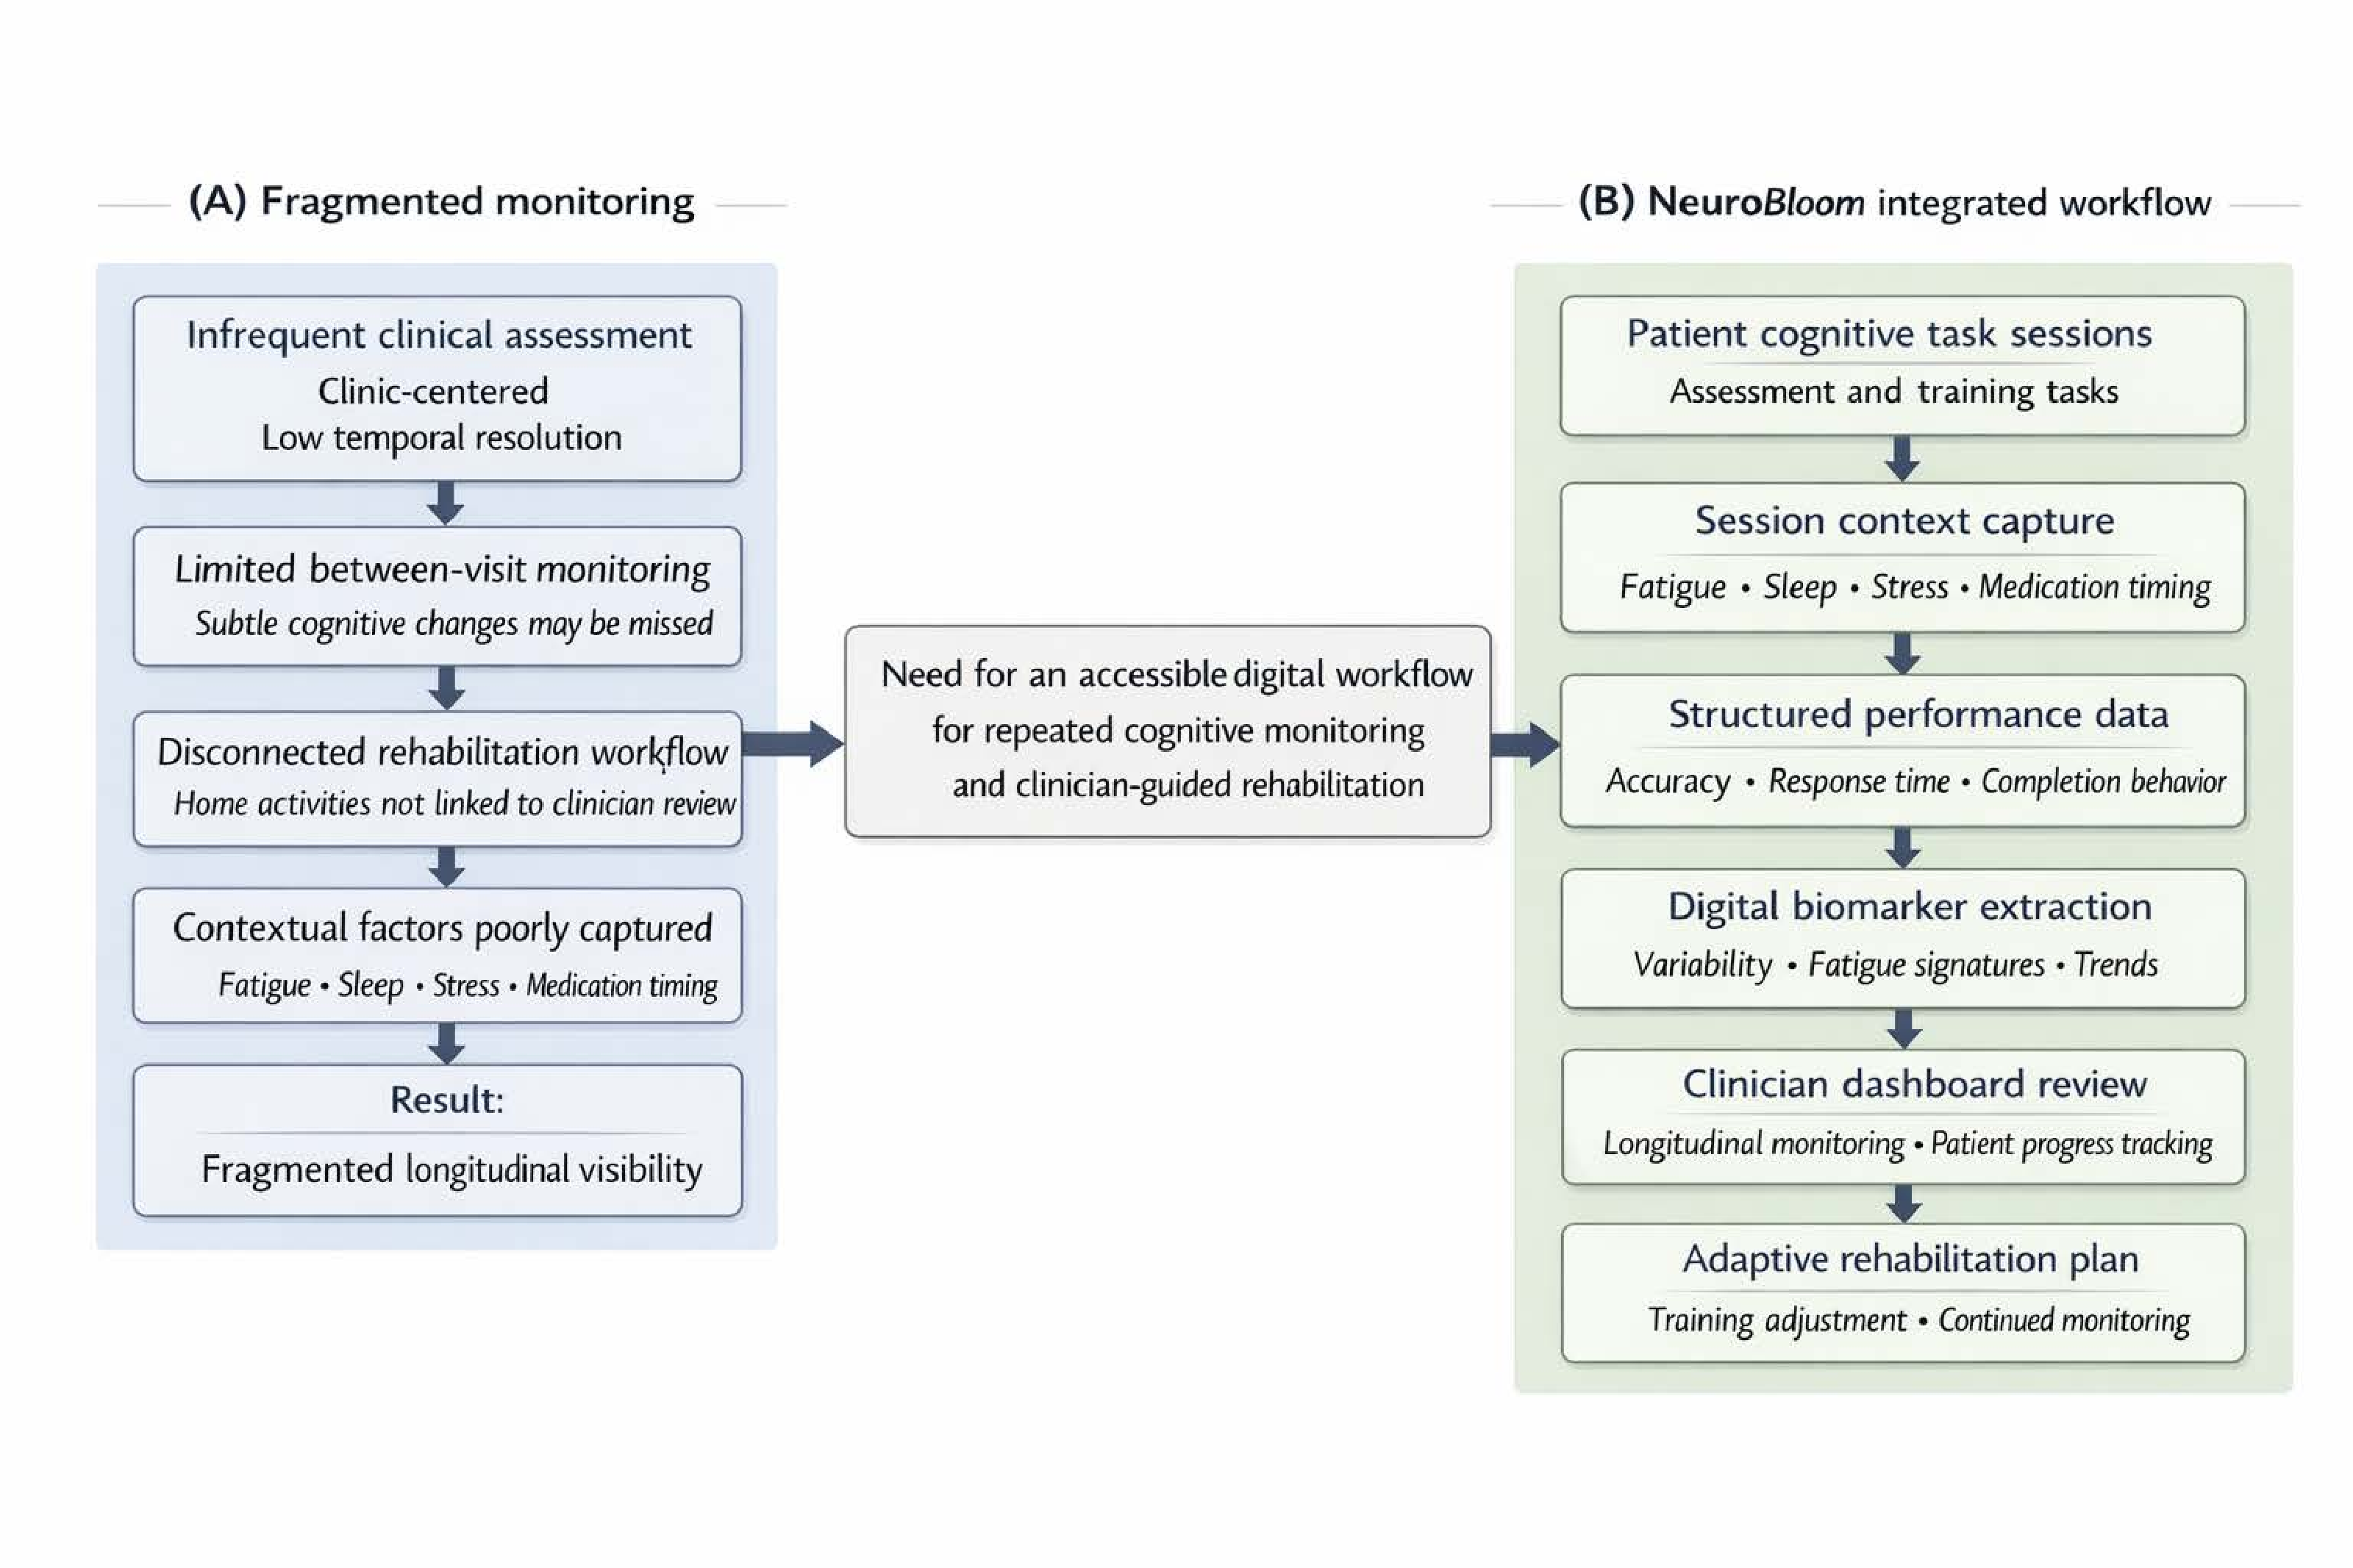
\includegraphics[width=\textwidth]{figure1}
\caption{Clinical motivation and integrated NeuroBloom workflow for repeated MS-oriented cognitive follow-up.}
\label{fig:motivation_workflow}
\end{figure}

NeuroBloom is designed as a free-of-cost, web-based platform for longitudinal cognitive monitoring and clinician-guided rehabilitation in multiple sclerosis. Rather than treating cognitive assessment as a collection of isolated task results, it supports repeated cognitive interaction, contextual data capture, and coordinated patient--clinician follow-up within a unified workflow. This allows performance to be observed over time across domains such as processing speed, working memory, attention, executive flexibility, planning, and visual scanning, while remaining practical for supervised rehabilitation and routine review. To improve accessibility across diverse user groups, NeuroBloom includes bilingual patient-facing support in Bangla and English, broadening usability in local and resource-constrained settings.

Because repeated interaction data can capture changes that may not be visible in single-session results, an additional motivation for NeuroBloom is the growing importance of digital biomarkers in neurorehabilitation and remote monitoring research \cite{insel2017,coravos2019,dorsey2017}. NeuroBloom includes an analytics layer that derives behavioral indicators from task interaction data and contextual information, including fatigue-related patterns, response-time variability, and trend measures across repeated sessions.These analytics function as review signals that help clinicians interpret patient progress and refine rehabilitation strategies over time.

The intended operational setting for NeuroBloom is therefore a coordinated digital follow-up workflow. A patient interacts with baseline or training tasks through the patient interface, optionally providing pre-session contextual information such as fatigue or sleep quality. Performance data are stored and analyzed over time, after which a clinician can review performance trends over time, assess adherence and task-level performance, and adjust prescriptions or training plans through the doctor portal. Administrative users support governed deployment, user management, and operational oversight. In this way, the software is designed not only for repeated patient interaction but also for integration into supervised rehabilitation and monitoring workflows.

Several elements of NeuroBloom build on established neuropsychological practice, including task paradigms relevant to processing speed, sustained attention, working memory, and executive function \cite{benedict2012,kalb2018}.Rather than introducing a standalone cognitive test, NeuroBloom contributes a unified digital platform that brings together repeated task interaction, contextual data capture, analytics-driven review, clinician-guided rehabilitation, and coordinated multi-role workflows. This makes the software relevant both as a practical tool for accessible MS follow-up and as a reusable framework for reproducible cognitive monitoring research.

\section{Software description}

NeuroBloom is a modular, role-based web platform for longitudinal cognitive monitoring and clinician-guided rehabilitation support in multiple sclerosis. It integrates 34 cognitive tasks across six domains into a standardized session model and combines patient-facing task execution with contextual data capture, clinician review workflows, administrative oversight, and a dedicated analytics layer within a unified software architecture. A personalized session planning and task-rotation mechanism regulates domain emphasis, task selection, and difficulty progression from baseline scores and ongoing rehabilitation priorities. Bilingual patient-facing support in Bangla and English broadens accessibility, and the modular design remains extensible to future task modules and analytical additions without restructuring the core system.

\subsection{Software architecture}
NeuroBloom is organized as a modular, role-aware architecture spanning three operational contexts—patient, doctor, and administrator. These contexts share a common backend and data model while preserving role-specific workflows. The system separates interface functions, core application services, analytics processing, and persistent storage, allowing different parts of the platform to evolve without disrupting the overall workflow.

At implementation level, NeuroBloom combines a Svelte-based frontend, a FastAPI backend, and a persistence layer built on SQLModel and PostgreSQL. The frontend provides role-specific interfaces for task execution, progress review, patient management, analytics, and administration. The backend manages authentication, baseline and training operations, session planning, reporting, messaging, notifications, and doctor--admin coordination. This layered organization separates interface behavior from service logic and storage responsibilities, making the system easier to maintain and extend as new task modules and platform features are introduced.

Bilingual support for Bangla and English is implemented through a custom internationalisation layer in the frontend. Locale preference is stored in the user account and initialized before client-side hydration to avoid layout shift at page load. A structured translation catalog manages interface strings, while numeric outputs are rendered using Unicode Bengali digits when Bangla is active. To preserve script consistency in patient-facing cognitive tasks, Latin letter stimuli are remapped to corresponding Bengali script characters without altering task structure or scoring logic. Bilingual support is currently limited to the patient-facing interface, whereas clinician and administrative views remain in English.

\begin{figure}[!t]
\centering
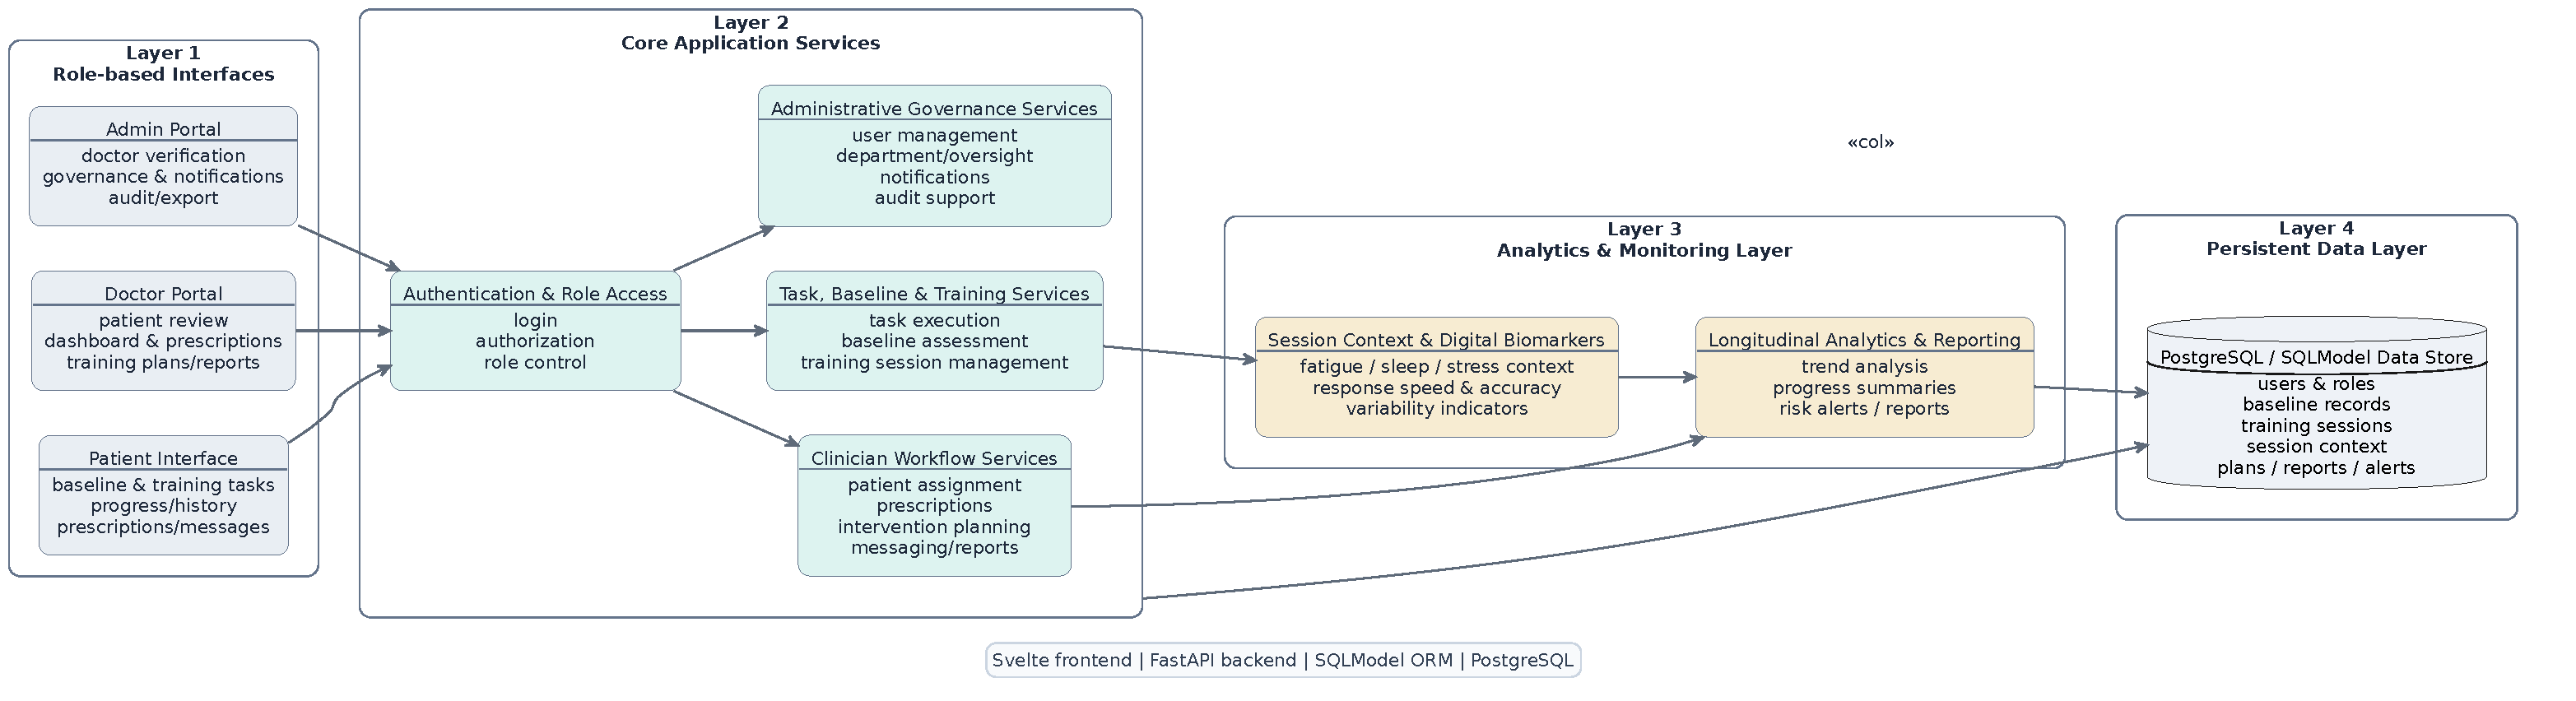
\includegraphics[width=\textwidth]{figure2}
\caption{Role-based system architecture of NeuroBloom, showing interface, service, analytics, and persistence layers.}
\label{fig:system_architecture}
\end{figure}

Data flow begins when a patient completes baseline or training activities and optionally submits contextual information such as fatigue, sleep quality, stress, or medication timing. These records are stored together with task outputs including score, accuracy, response time, completion behavior, and associated contextual variables. The resulting session history supports repeated review by clinicians and administrators, allowing patient performance to be interpreted across sessions rather than as isolated task results.

A task-planning component operates within the application layer to regulate session composition and progression. Using baseline scores, recent task history, and current difficulty levels, it determines domain emphasis, rotates task selection, and updates difficulty across repeated sessions. This enables NeuroBloom to function not merely as a repository of cognitive tasks, but as an adaptive rehabilitation workflow.


An analytics layer operates on stored session and trial records as a monitoring pipeline. Rather than functioning as a standalone diagnostic engine, it derives interpretable variability-, fatigue-, and trend-related measures for clinician-facing review. The processing sequence linking task interaction, contextual capture, and biomarker-oriented summaries is illustrated in Fig.~\ref{fig:biomarker_pipeline}.
.

\begin{figure}[!htbp]
\centering
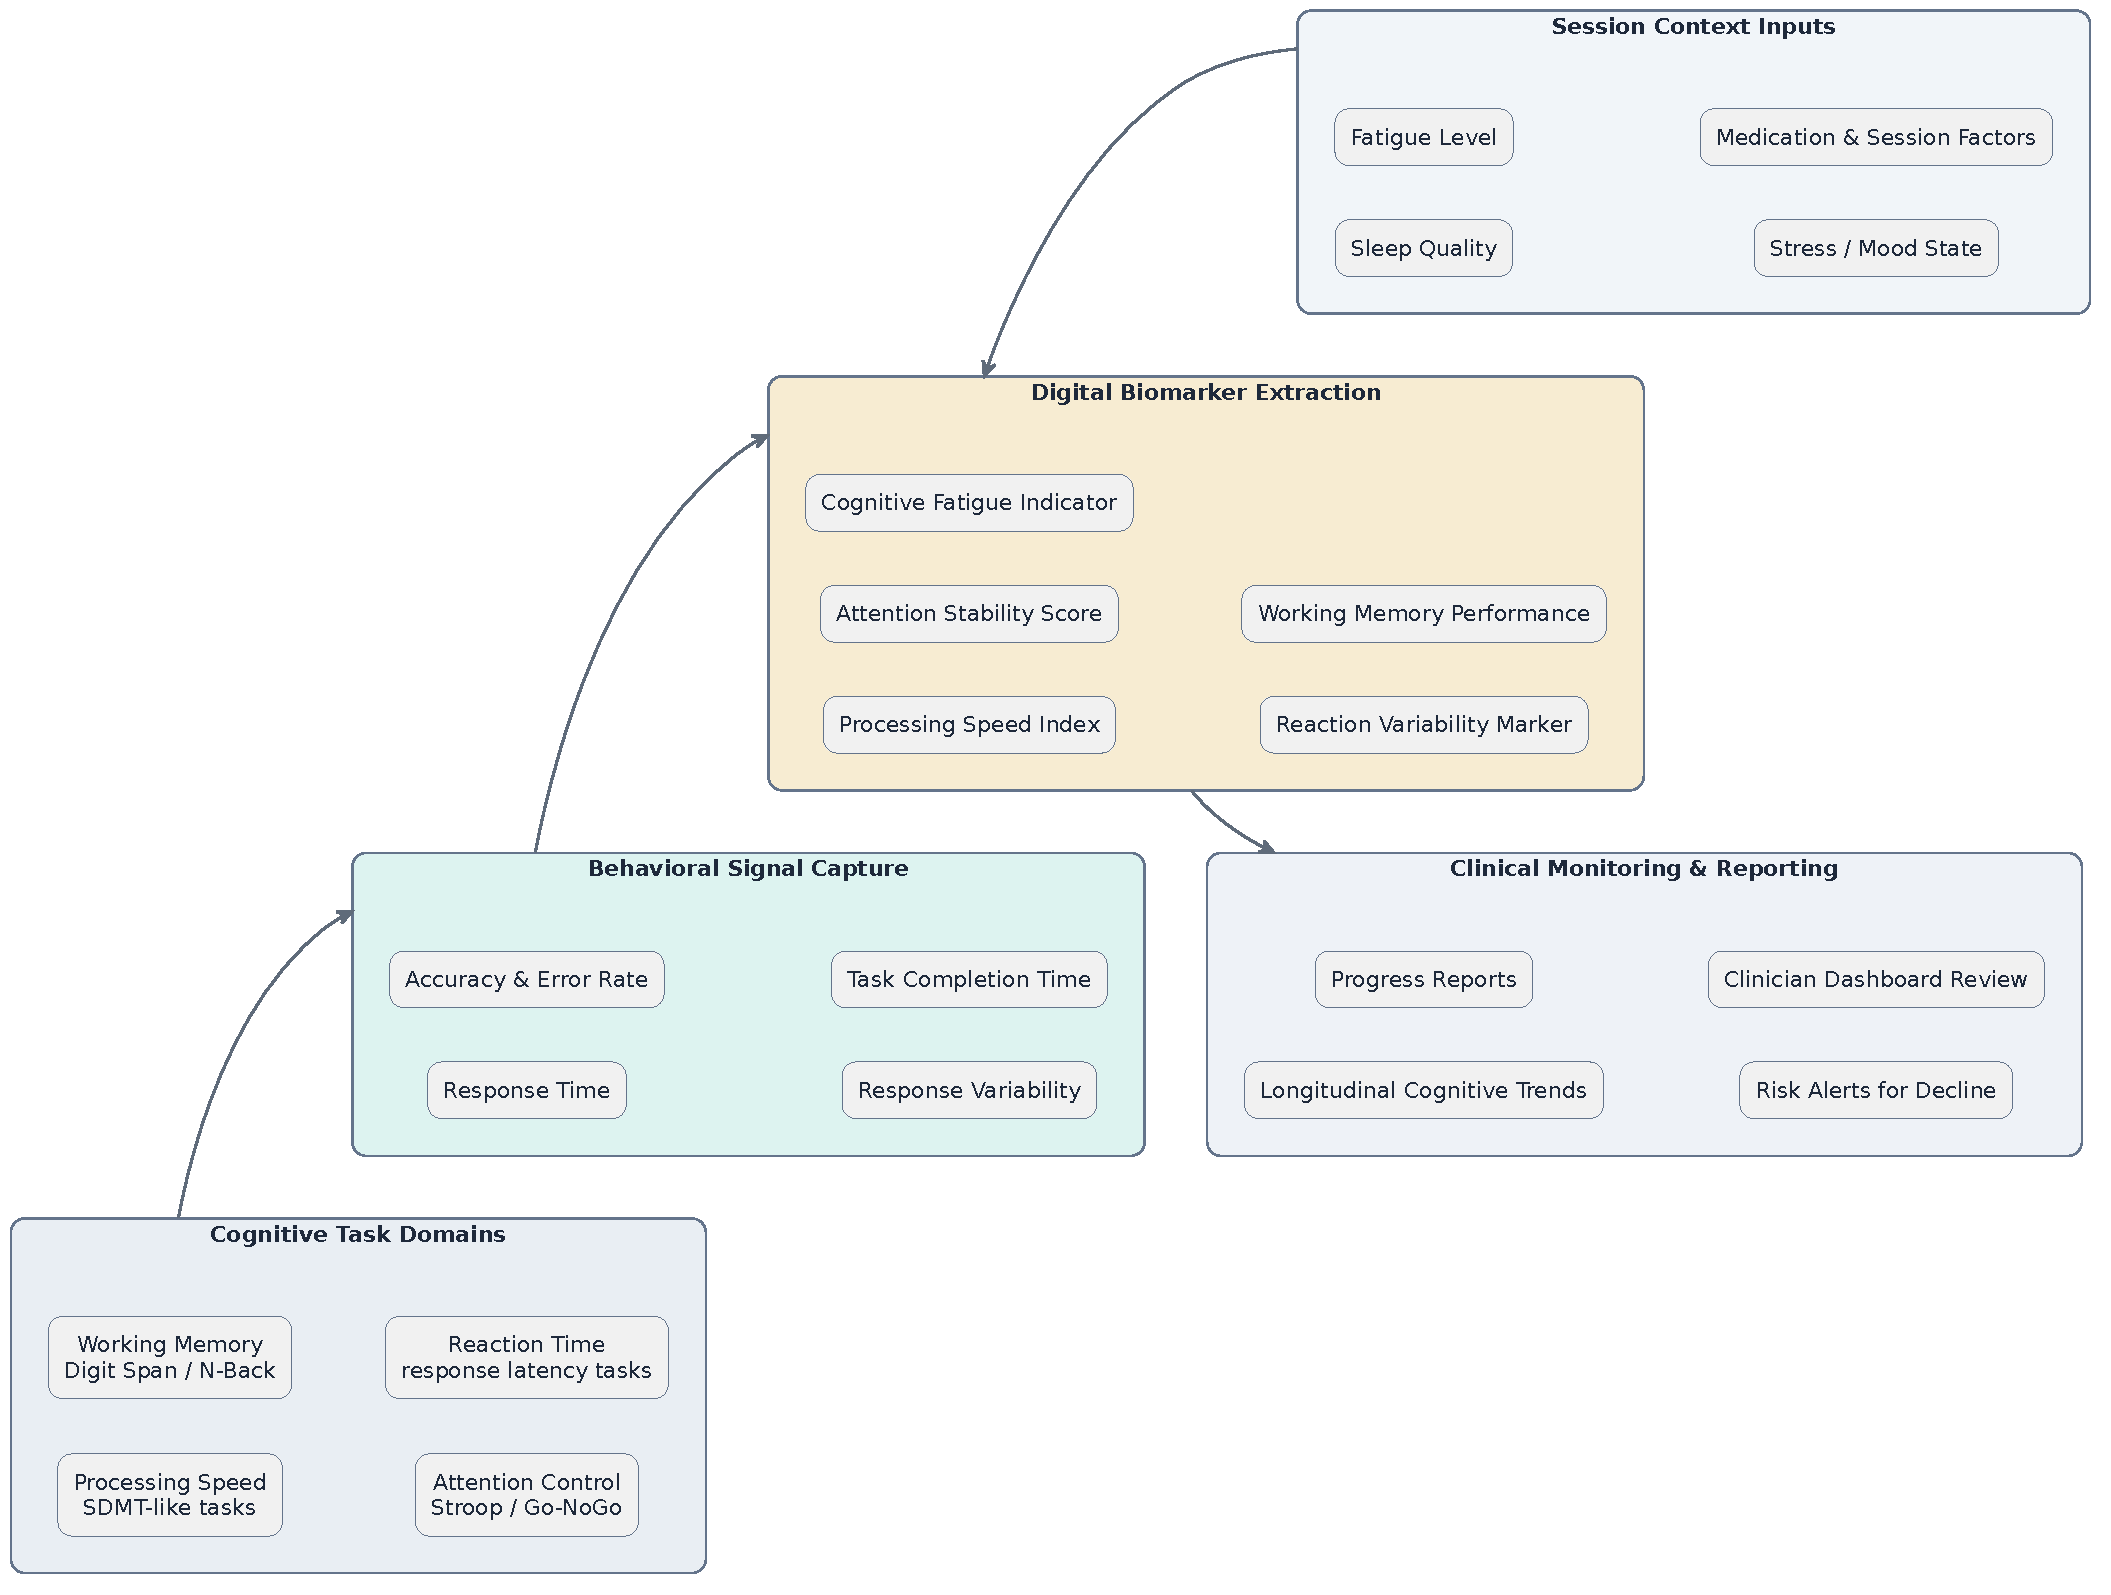
\includegraphics[width=\textwidth]{figure3}
\caption{Analytics pipeline linking task interaction and contextual capture to longitudinal summaries and biomarker-oriented outputs.}
\label{fig:biomarker_pipeline}
\end{figure}

This layered separation enables controlled role-based access, supports reuse of shared data structures, and allows the platform to evolve without redesigning the full system. In this way, the architecture provides a practical basis for reproducible data capture, adaptive rehabilitation support, and coordinated clinician--patient interaction.


\subsection{Software functionalities}
\paragraph{Patient interaction and session execution}
Patient interaction and session execution. NeuroBloom provides a patient-facing workflow for repeated baseline and training activity. Patients complete structured cognitive tasks, view session progress, and optionally submit pre-session contextual information such as fatigue or sleep quality, supporting adherence-oriented use across home- or clinic-based follow-up. To improve accessibility, the patient interface is available in both Bangla and English. The interaction flow is illustrated in Fig.~\ref{fig:patient_workflow}.

\begin{figure}[!t]
\centering
\begin{minipage}[t]{0.40\textwidth}
\centering
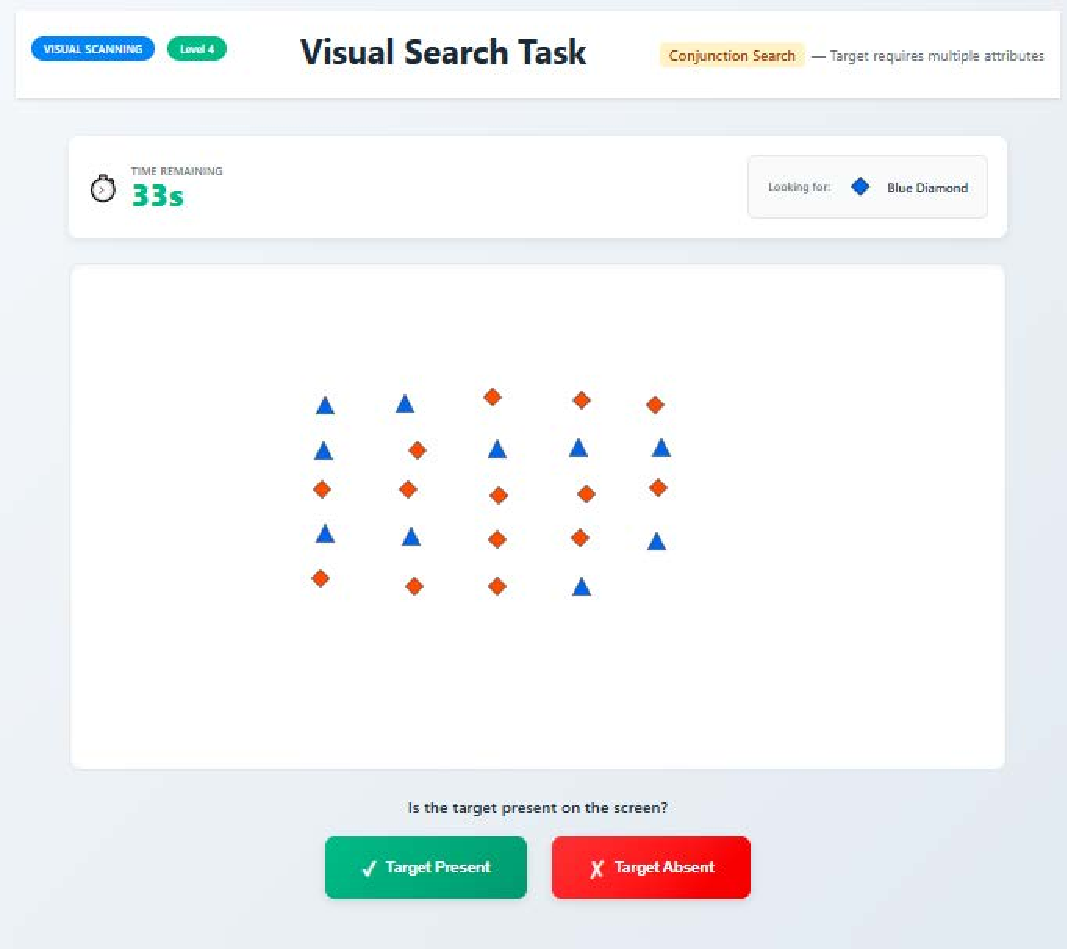
\includegraphics[width=0.90\linewidth]{fig4part1}\\[-0.3em]
{\small (a)}
\end{minipage}\hfill
\begin{minipage}[t]{0.40\textwidth}
\centering
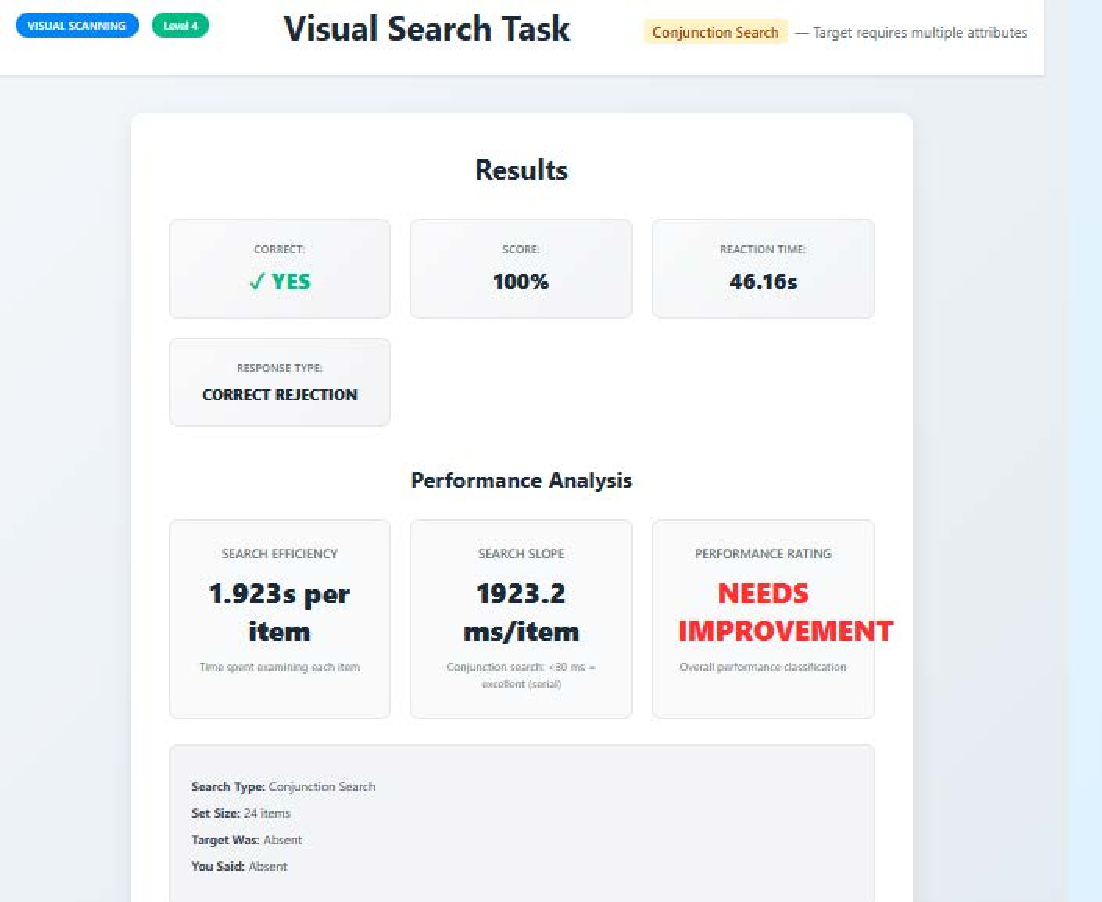
\includegraphics[width=0.90\linewidth]{fig4part2}\\[-0.3em]
{\small (b)}
\end{minipage}

\vspace{0.3em}

\begin{minipage}[t]{0.40\textwidth}
\centering
\includegraphics[width=0.90\linewidth]{figure4_3}\\[-0.3em]
{\small (c)}
\end{minipage}\hfill
\begin{minipage}[t]{0.40\textwidth}
\centering
\includegraphics[width=0.90\linewidth]{figure4_4}\\[-0.3em]
{\small (d)}
\end{minipage}
\caption{Patient-facing workflow in NeuroBloom. (a)--(b) English interface showing repeated task interaction and progress-oriented session use. (c)--(d) Equivalent Bangla interface, illustrating bilingual patient-facing support.}
\label{fig:patient_workflow}
\end{figure}

\paragraph{Cognitive task framework}
The task framework includes 34 tests across six cognitive domains—working memory, processing speed, attention, cognitive flexibility, planning, and visual scanning—integrated into a common session model that standardizes outputs including score, accuracy, response speed, completion behavior, and difficulty-linked progression. Each task spans 10 difficulty levels for adaptive progression, and a session-level selection mechanism emphasizes domains aligned with each patient's weaker or more rehabilitation-relevant areas.

\begin{center}
\begin{minipage}{0.92\linewidth}
\small
\textbf{Algorithm 1. Personalized session planning and task rotation in NeuroBloom}
\begin{algorithmic}[1]
\Require Baseline scores $B[d]$, recent task history $H[d]$, current difficulties $L[d]$
\State $\textit{sorted\_domains} \gets \Call{SortAscending}{B}$
\State $\textit{primary\_focus} \gets \textit{sorted\_domains}[0:2]$
\State $\textit{secondary\_focus} \gets \textit{sorted\_domains}[2:4]$
\State $\textit{maintenance} \gets \textit{sorted\_domains}[4:6]$
\ForAll{domain $d$ in $B$}
    \State $L[d] \gets \Call{ScoreToDifficulty}{B[d]}$
\EndFor
\State $\textit{session\_domains} \gets \textit{primary\_focus} \cup \textit{secondary\_focus}$
\ForAll{domain $d$ in $\textit{session\_domains}$}
    \State $\textit{available} \gets \Call{GetAvailableTasks}{d}$
    \State $\textit{recent} \gets \Call{GetRecentTasks}{H[d], d}$
    \State $\textit{candidates} \gets \Call{ExcludeRecentWhenPossible}{\textit{available}, \textit{recent}}$
    \State $\textit{strategy} \gets \Call{RotationStrategy}{d}$
    \State $\textit{task}[d] \gets \Call{SelectTask}{\textit{candidates}, \textit{strategy}, L[d]}$
\EndFor
\ForAll{completed task result $r$}
    \State \Call{StoreTrainingSession}{$r$}
    \State $L[r.domain] \gets \Call{UpdateDifficulty}{L[r.domain], r.score, r.accuracy, r.reaction\_time}$
\EndFor
\If{\Call{ShouldRebalanceFocusAreas}{active training plan}}
    \State \Call{RebalanceFocusAreas}{active training plan}
\EndIf
\State \Return personalized four-task session plan
\end{algorithmic}
\end{minipage}
\end{center}

\paragraph{Longitudinal analytics and digital biomarkers}
Beyond raw task completion, the platform derives summary analytics from accumulated performance and contextual records, including longitudinal trend summaries, fatigue-related patterns, and response-time variability indicators. These outputs support progression-aware monitoring and clinician interpretation of rehabilitation-relevant change. The processing pipeline is illustrated in Fig.~\ref{fig:biomarker_pipeline}; an example dashboard is shown in Fig.~\ref{fig:admin_workflow}(a).

The current analytics layer is based on deterministic statistical feature extraction. All indicators are computed directly from trial-level accuracy, reaction times, session-level scores, and contextual self-report variables. Within-session cognitive fatigue is estimated from the difference between early- and late-session performance, with
\begin{equation}
\Delta Acc = Acc_{Q1} - Acc_{Q4}, \qquad \Delta RT = RT_{Q4} - RT_{Q1},
\end{equation}
where $Q1$ and $Q4$ denote the first and last quartiles of trials in a session. A trial-wise linear slope $\beta$ of accuracy over time is also computed, and the normalized fatigue index is defined as
\begin{equation}
F = 0.5A + 0.3R + 0.2S,
\end{equation}
where $A=\min(1,\max(0,\Delta Acc/30))$, $R=\min(1,\max(0,\Delta RT/200))$, and $S=\min(1,\max(0,-100\beta))$.

Reaction-time variability is summarized using a suite of intra-individual variability (IIV) measures. The primary measure is the coefficient of variation,
\begin{equation}
CV = \frac{\sigma_{RT}}{\mu_{RT}},
\end{equation}
where $\sigma_{RT}$ and $\mu_{RT}$ are the standard deviation and mean of valid reaction times. Complementary robust measures---median absolute deviation (MAD), interquartile range (IQR), and full range---are also computed to characterize distributional spread independently of outliers. Elevated IIV has been associated with white matter lesion load and functional impairment in MS, making these measures clinically relevant monitoring outputs.

For longitudinal monitoring, NeuroBloom applies an exponentially weighted moving average (EWMA) to repeated performance values:
\begin{equation}
EWMA_t = \alpha x_t + (1-\alpha)EWMA_{t-1},
\end{equation}
with $\alpha=0.2$ in the current implementation. Trend direction (improving, stable, or declining) and trend strength are derived from the slope of the five most recent EWMA points and are surfaced in the clinician-facing review interface. Across sessions, score change is also summarized using a reliable change index,
\begin{equation}
RCI = \frac{X_{\mathrm{latest}} - X_{\mathrm{baseline}}}{\sqrt{2}\,\sigma_X},
\end{equation}
where $\sigma_X$ is the observed standard deviation of session scores for the individual. Associations between contextual variables---including fatigue level, sleep quality, hours since medication, stress level, pain level, and readiness level---are estimated using Pearson correlation coefficients with session score and mean reaction time. These indicators are intended as heuristic monitoring features and longitudinal summary measures, not as validated diagnostic biomarkers or predictive clinical models.

\paragraph{Doctor-facing clinical workflow}
The clinician-facing functionality connects patient interaction data to supervised review and intervention. Doctors can inspect patient histories, assess adherence and recent performance, review biomarker-oriented summaries and trend information, generate or review progress reports, and modify training plans, task difficulty levels, or prescriptions in response to observed change. By linking monitoring outputs to concrete clinical actions, the software supports iterative rehabilitation management rather than passive data display alone. The doctor-facing review and intervention process is shown in Fig.~\ref{fig:doctor_workflow}.

\begin{figure}[!t]
\centering
\begin{minipage}[t]{0.49\textwidth}
\centering
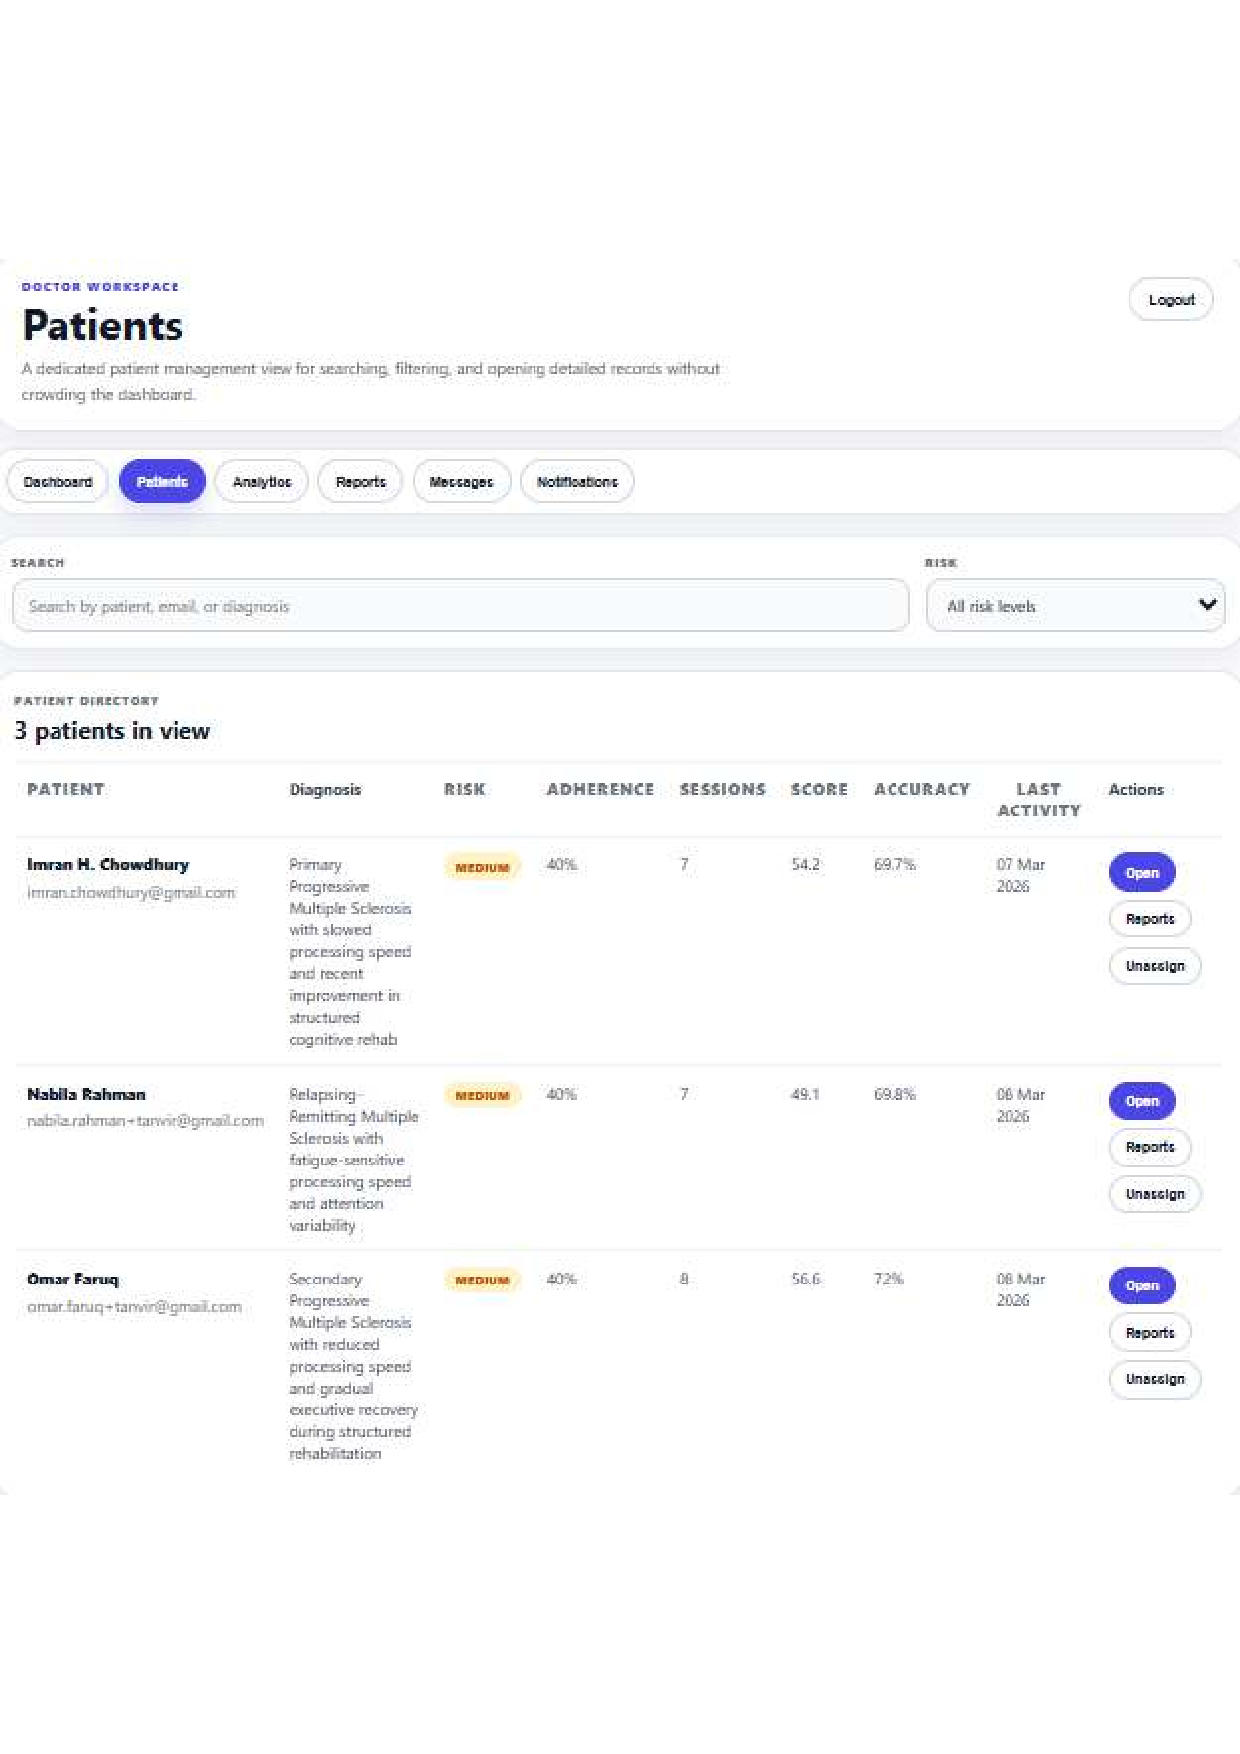
\includegraphics[width=\textwidth]{fig5part1}
\end{minipage}\hfill
\begin{minipage}[t]{0.49\textwidth}
\centering
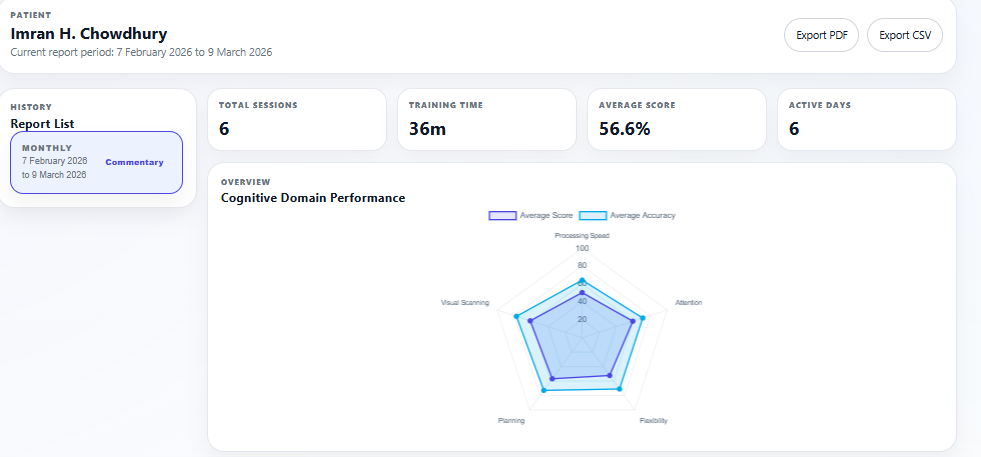
\includegraphics[width=\textwidth]{fig5part2}
\end{minipage}
\caption{Doctor-facing workflow, combining patient review, longitudinal monitoring, and intervention-oriented decision support.}
\label{fig:doctor_workflow}
\end{figure}

\paragraph{Administrative oversight and governance}
NeuroBloom also includes administrative functionality for governed deployment and operational supervision in a multi-user setting. Administrative users can review system-level activity, monitor engagement and alert-oriented summaries, manage user and role relationships, and maintain oversight of the platform as a coordinated service rather than a standalone task interface. This administrative layer is important because the software is intended to function as a managed rehabilitation and monitoring environment involving patients, clinicians, and institutional oversight. The administrative overview interface is illustrated in Fig.~\ref{fig:admin_workflow}(b).

\begin{figure}[!t]
\centering
\begin{minipage}[t]{0.49\textwidth}
\centering
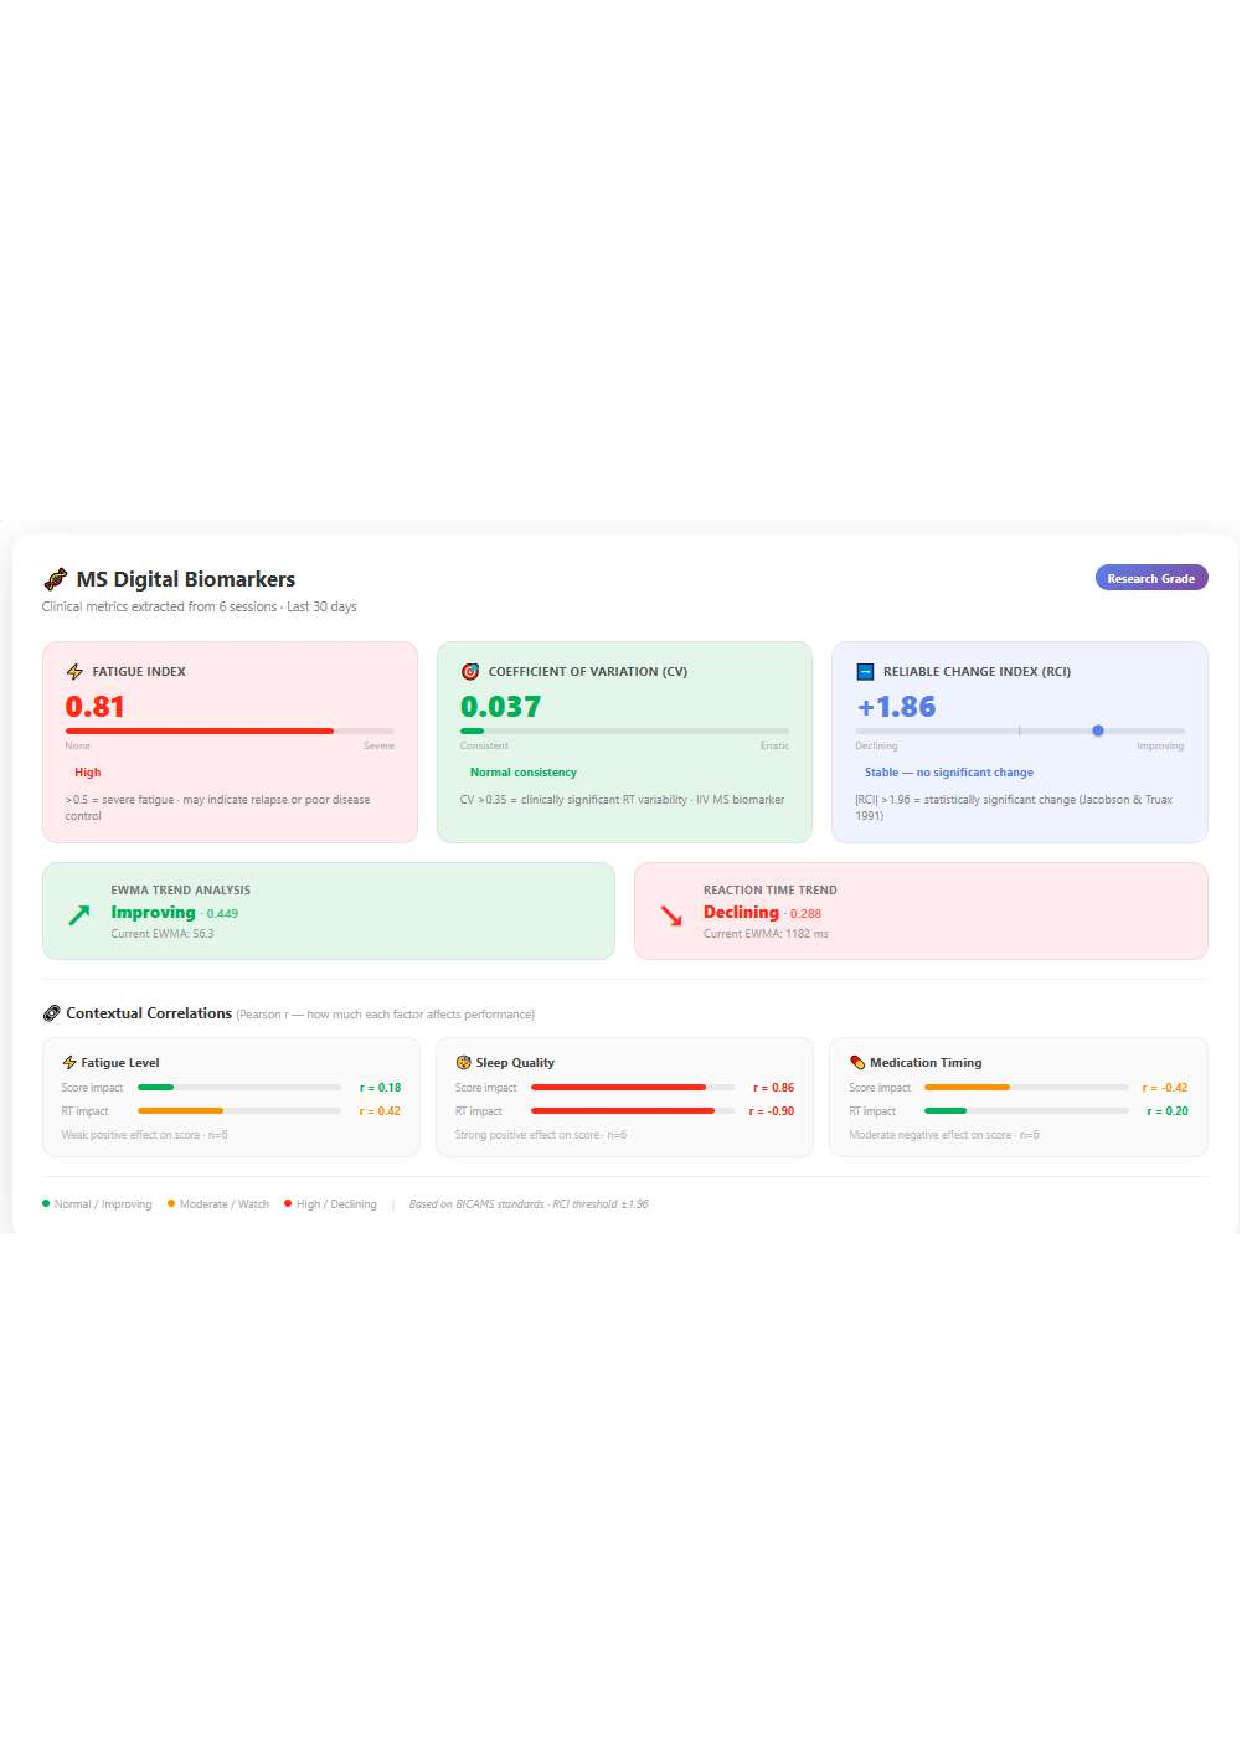
\includegraphics[width=\textwidth]{fig6part1}\\[-0.2em]
{\small (a)}
\end{minipage}\hfill
\begin{minipage}[t]{0.49\textwidth}
\centering
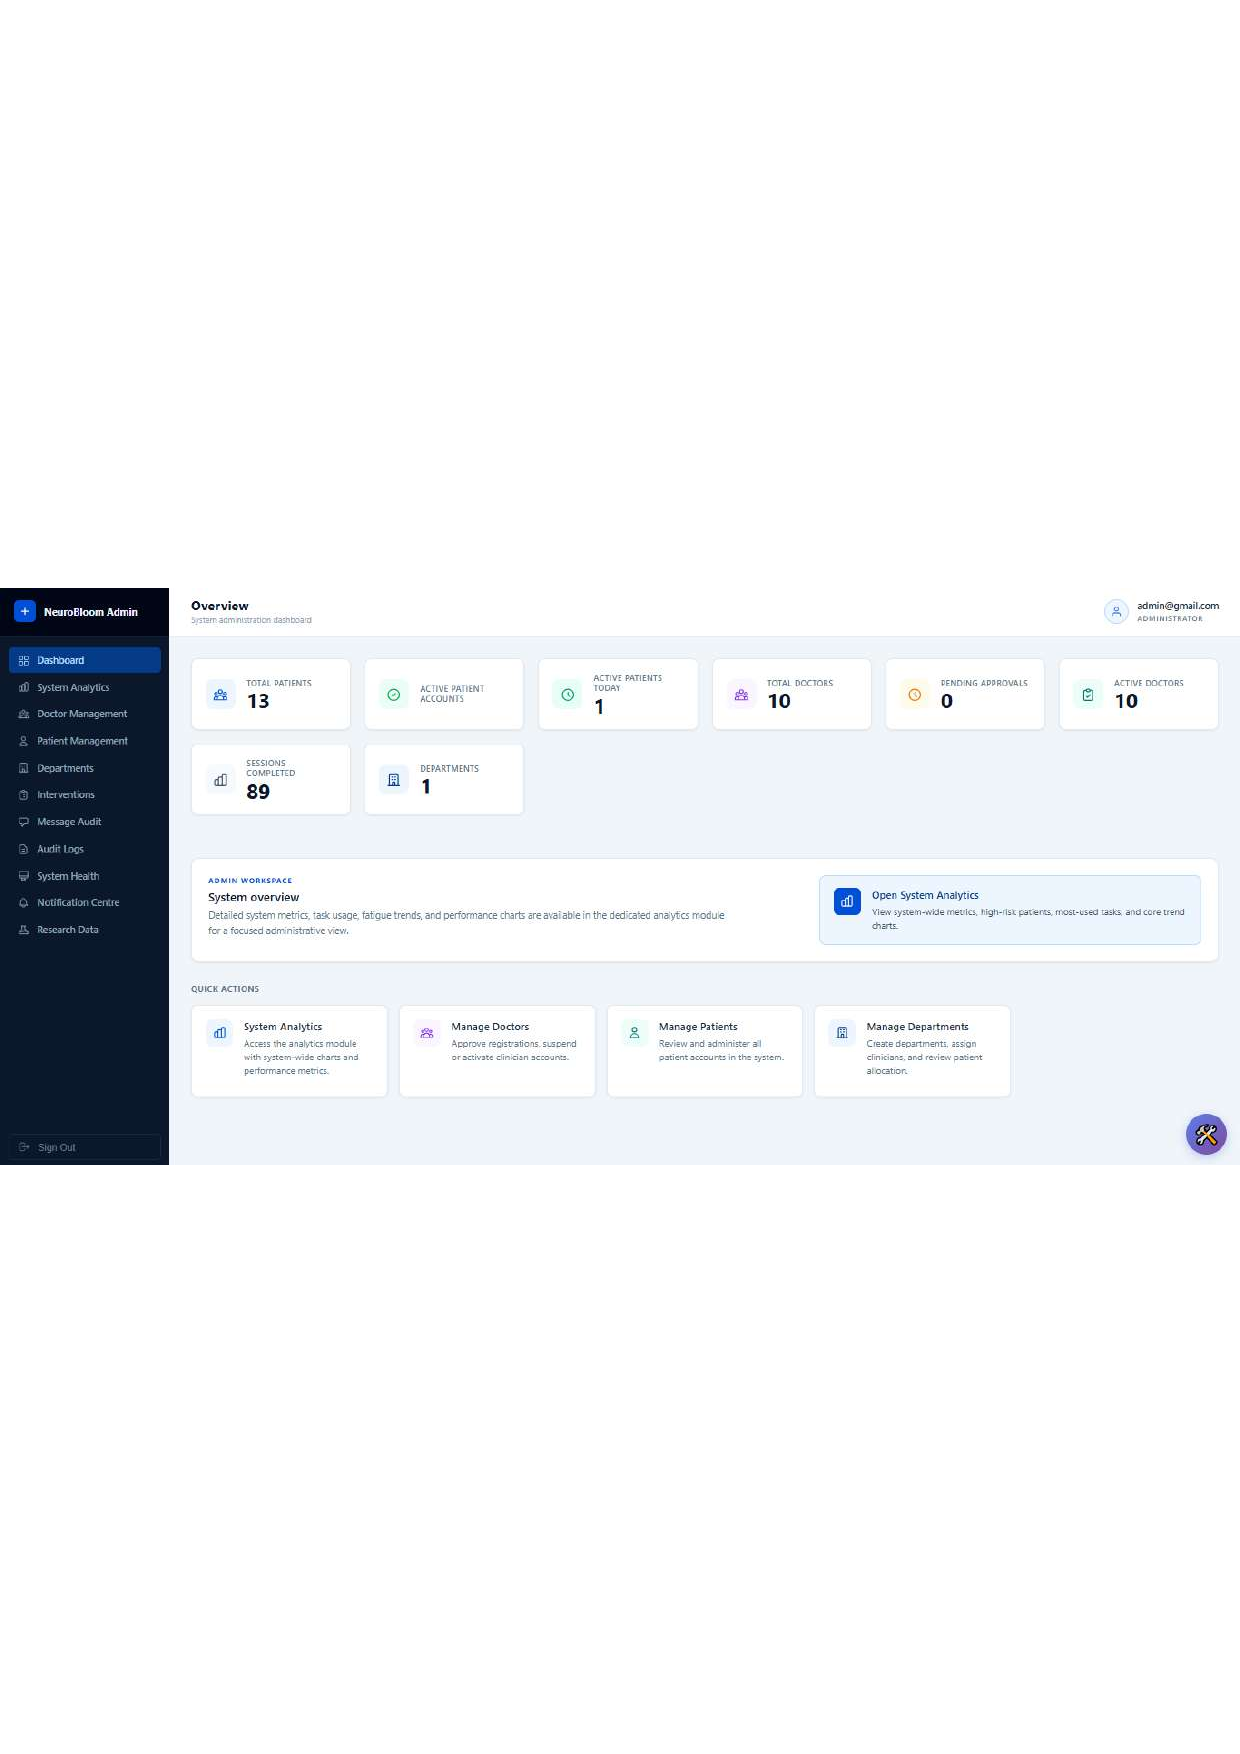
\includegraphics[width=\textwidth]{fig6part2}\\[-0.2em]
{\small (b)}
\end{minipage}
\caption{Analytics and administration views in NeuroBloom. (a) Biomarker and contextual analytics dashboard. (b) Administrative overview for system monitoring and governance.}
\label{fig:admin_workflow}
\end{figure}

\section{Illustrative examples}
To better demonstrate the major functions of the software, a supplementary video is provided showing the end-to-end operation of NeuroBloom. The video presents the principal patient, doctor, and administrative workflows and complements Figs.~\ref{fig:patient_workflow}--\ref{fig:admin_workflow} by illustrating how the main modules described in this article are used in practice.


\section{Impact}
NeuroBloom contributes a research-oriented software environment for cognitive monitoring and rehabilitation-related data collection in multiple sclerosis. By combining repeated task execution, contextual self-report capture, and persistent session history within a unified platform, the system supports structured investigation of behavioral change across sessions rather than isolated one-time measurement. This makes the software relevant for studies of digital behavioral indicators, repeated cognitive interaction, and the influence of contextual factors such as fatigue or sleep quality on performance \cite{insel2017,coravos2019}.

The platform also has practical value for MS-oriented follow-up between formal clinical encounters. In addition to collecting patient-side task and context data, NeuroBloom closes the feedback loop between patient activity and clinician response by linking repeated task execution to doctor-facing review tools, summary analytics, progress reporting, and rehabilitation adjustment. This coordinated workflow supports low-cost, supervision-oriented follow-up while reducing barriers to access through a free-of-cost deployment model, particularly in resource-constrained settings where both specialist review and repeated access to diagnostic resources such as MRI and laboratory testing may be limited.

From a software perspective, NeuroBloom provides a modular and extensible architecture that integrates cognitive task delivery, contextual data capture, analytics, adaptive session planning, and multi-role workflow management within a single system. This design supports reuse of the platform as a research and deployment framework, allowing additional task modules, analytics components, and reporting workflows to be incorporated without restructuring the core architecture. Because its analytics layer is based on interpretable statistical indicators and its task-planning workflow is explicitly defined, NeuroBloom also supports transparent, reproducible, and extensible digital monitoring research.

\section{Conclusions}
NeuroBloom establishes a modular, web-based framework for longitudinal cognitive monitoring and clinician-supervised rehabilitation in multiple sclerosis. By unifying task-based assessment with contextual data capture and adaptive session planning, the platform provides a structured environment for identifying behavioral trends that are often missed in traditional clinical encounters. Its decoupled architecture and bilingual support make it a practical, reproducible foundation for digital health research and clinical follow-up, particularly in resource-constrained settings. Future work will focus on large-scale deployment to evaluate longitudinal user engagement, the expansion of the task library, and the refinement of predictive analytics to further support clinician-led rehabilitation decisions.

\section*{Acknowledgements}
TODO

\section*{Declaration of Generative AI and AI-assisted technologies in the writing process}
During the preparation of this work the authors used AI tools in order to improve the readability and language of the manuscript. After using this service, the authors reviewed and edited the content as needed and take full responsibility for the content of the published article.

\section*{Declaration of competing interest}
TODO

\begin{thebibliography}{00}

\bibitem{chiaravalloti2008} N.D. Chiaravalloti, J. DeLuca, Cognitive impairment in multiple sclerosis, Lancet Neurol. 7 (2008) 1139--1151.

\bibitem{amato2006} M.P. Amato, V. Zipoli, E. Portaccio, Multiple sclerosis-related cognitive changes: a review of cross-sectional and longitudinal studies, J. Neurol. Sci. 245 (2006) 41--46.

\bibitem{rocca2015} M.A. Rocca, M.P. Amato, N. De Stefano, et al., Clinical and imaging assessment of cognitive dysfunction in multiple sclerosis, Lancet Neurol. 14 (2015) 302--317.

\bibitem{kalb2018} R. Kalb, T. Beier, R.H.B. Benedict, et al., Recommendations for cognitive screening and management in multiple sclerosis care, Mult. Scler. J. 24 (2018) 1665--1680.

\bibitem{benedict2012} R.H.B. Benedict, M.P. Amato, J. Boringa, et al., Brief International Cognitive Assessment for Multiple Sclerosis (BICAMS): international standards for validation, BMC Neurol. 12 (2012) 55.

\bibitem{insel2017} T.R. Insel, Digital phenotyping: technology for a new science of behavior, JAMA 318 (2017) 1215--1216.

\bibitem{coravos2019} A. Coravos, S. Khozin, K.D. Mandl, Developing and adopting safe and effective digital biomarkers to improve patient outcomes, npj Digit. Med. 2 (2019) 14.

\bibitem{dorsey2017} E.R. Dorsey, S. Papapetropoulos, M. Xiong, K. Kieburtz, The first frontier: digital biomarkers for neurodegenerative disorders, Digit. Biomark. 1 (2017) 6--13.

\end{thebibliography}

\end{document}
